\chapter{Line, Circle, Cylinder and Sphere}
\lecture{5}{9 May. 00:51}{Fifth Lecture}
\label{chap:something}

\section{Straight Lines in Polar Form}
\label{sec:straight-lines-in-polar-form}

In Cartesian Coordinate system, a straight line can be representation in many
form. One of them is slope form \( y = mx + c \). But the one that mostly
relates with Polar System is the normal form of representing a straight line.

\begin{figure}[H]
  \centering
  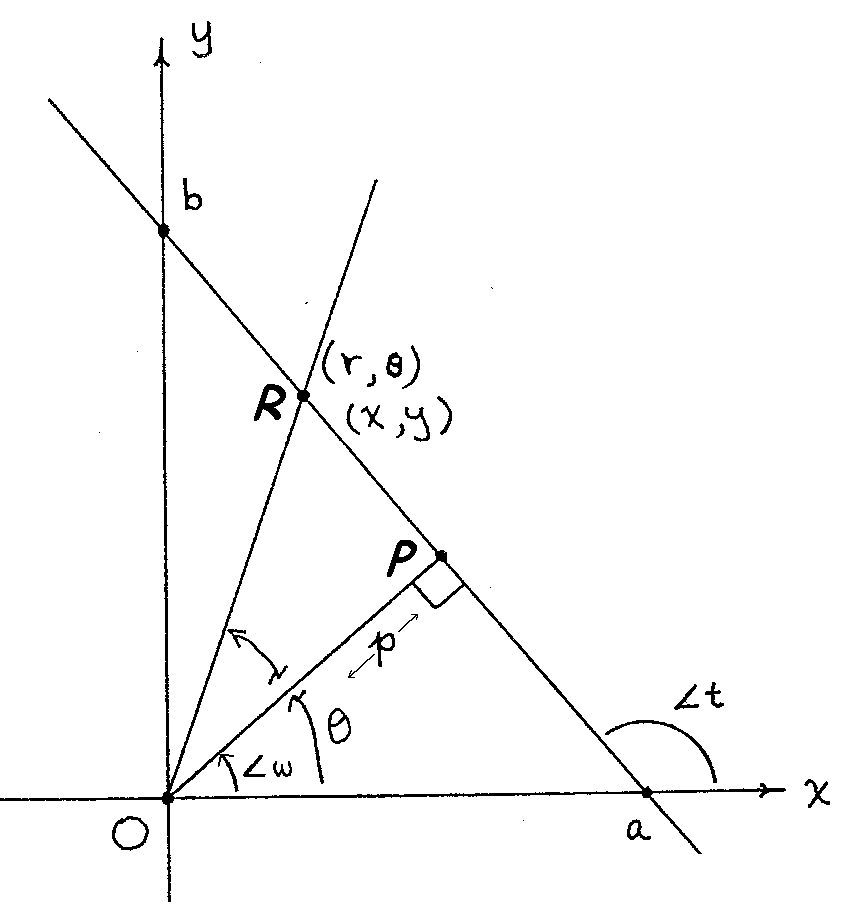
\includegraphics[width=0.8\textwidth]{Figures/pimg1.png}
  \caption{Figure for derivation of Straight Line}
  \label{fig:pimg1}
\end{figure}

\begin{equation}
  \label{eqn:normal-form-straight-line}
  \begin{displaystyle}
    x \cos(\alpha) + y \sin(\alpha) = r_{o}
  \end{displaystyle}
\end{equation}
Now we subsititute the value of x and y so that the equation becomes: 
\[ r\cos\theta\cos\theta_o+r\sin(\theta)\sin(\theta_o) =r_o\] 
\begin{center}
  \begin{equation}
    \begin{displaystyle}
      r_o = r(\cos(\theta-\theta_o))
    \end{displaystyle}
    \label{eqn:polar-form-straight-line}
  \end{equation}
\end{center}
\begin{note}
  Here, \(r_o\) is the \href{sec:polar-coord-syst}{radial coordinate} of the
  point of intersection between the perpendicular to the line in question from the origin.
\end{note}

\section{Equation of a Circle in Polar Form}
\label{sec:equation-of-a-cirle-in-polar-form}

% TODO: Fig for equation of circle

From above figure, Using cosine law on triange \ldots,
\[ 
  \cos(\theta-\theta_o) = \frac{r^{2}+{r_o}^2-a^2}{2rr_o}
\]
\begin{equation}
  \label{eqn:cirle-in-polar-form}
  \begin{displaystyle}
    \therefore\quad r^2+{r_o}^2-2rr_o\cos(\theta-\theta_o) = a^2
  \end{displaystyle}
\end{equation}

\subsection{Different cases of Circle}
\label{ssec:different-cases-of-circle}
% TODO: Add desmos play.

\paragraph{Circle passes through pole}
\begin{equation}
  \label{eqn:circle-passes-through-pole}
  \begin{displaystyle}
    r^2 = 2ar\cos(\theta-\theta_o)
  \end{displaystyle}
\end{equation}

\paragraph{Circle passes through pole and center in x-axis}
Here, \(\theta_o=0\).
Then from \autoref{eqn:circle-passes-through-pole},
\[ r = 2a\cos\theta \] where, \(a \in \Z\).

\paragraph{Circle passes through pole and center in y-axis}
Here, \(\theta_o=\frac{\pi}{2}\).
Then from \autoref{eqn:circle-passes-through-pole},
\[ r = 2a\sin\theta \] where, \(a \in \Z\).

\paragraph{Circle and center at pole}
Here, \(r=0\).
Then from \autoref{eqn:cirle-in-polar-form},
\[ r = a \] where, \(a \in \Z\).

\section{Cylindrical Coordinates}
\label{sec:cylindrical-coordinates}

A point in cylindrical coordinate system is represented with
\((r,\theta,z)\).\\
where \((r,\theta)\) is the point in \emph{x-y plane} And \(z\) is the
translation of that point in the z-direction.

% TODO: Play with it.

\subsection{Some Useful Equations}
\label{ssec:some-useful-equations}
\begin{itemize}
  \item \(r=a\) represents a cylinder with infinite height and depth.\\
  \item \(\theta=\theta_o\) represents a plane containing z-axis.\\
  \item \(z=z_o\) represents a plane roof parallel to \emph{x-y plane}.
  \item \(z=r^2\) represents a \textbf{paraboloid}. 
  \item \(z=r\) represents a cone.
\end{itemize}
% TODO: Play with it.
% TODO: examples

\section{Spherical Coordinates}
\label{sec:spherical-coordinates}
% TODO: Play and figure.

A point in spherical coordinate system is represented with
\((\rho,\phi,\theta)\).\\
where,\\
\(\rho\) is the distance of the point from the pole.\\
\(\phi\) is the angle between the projection of the line (joining pole to our
point) in the \emph{y-z plane} and the z-axis.\\
\(\theta\) is the angle between the projection of the line (joining pole to
our point) in the \emph{x-y plane} and the x-axis.


% TODO: Play with it.

\subsection{Some Useful Equations}
\label{ssec:some-useful-equations}
\begin{itemize}
  \item \(\rho=a\) \(\rightarrow\) Sphere
  \item \(\phi=\phi_o\) \(\rightarrow\) Cone
    \begin{itemize}
      \item \(\phi_o = \frac{\pi}{2}\) \(\rightarrow\) \emph{x-y plane}
      \item \(\phi_o = 0\) \(\rightarrow\) \emph{+ve z-axis}
      \item \(\phi_o = \pi\) \(\rightarrow\) \emph{-ve z-axis}
      \item \(0<\phi_o<\frac{\pi}{2}\) \(\rightarrow\) cone, widens at
        \(2\phi_o\) angle in the positive z direction.
      \item \(\frac{\pi}{2}<\phi_o<\pi\) \(\rightarrow\) cone, widens at
        \(2(\pi-\phi_o)\) angle in the negative z direction.
    \end{itemize}
  \item \(\theta=\theta_o\) \(\rightarrow\) plane containing z-axis.
\end{itemize}


% TODO: Play with it.

% TODO: examples
